\documentclass[11pt]{article} % 
\usepackage[pdftex]{graphicx}
\usepackage{fullpage}
\usepackage{graphicx}
\usepackage{graphics}
\usepackage{psfrag}
\usepackage{pgf}
\usepackage{color}
\usepackage{tikz}
\usetikzlibrary{arrows,automata}
\usepackage[latin1]{inputenc}
\usepackage{amsthm}
\usepackage{amsmath,amssymb}
\usepackage{enumerate}
\setlength{\textwidth}{6.5in}
\setlength{\textheight}{9in}
\newcommand{\N}{\mathbb{N}}
\newcommand{\Z}{\mathbb{Z}}
\newcommand{\R}{\mathbb{R}}
\newcommand{\Q}{\mathbb{Q}}
\newcommand{\C}{\mathbb{C}}
\newcommand{\PP}{\mathbb{P}}
\newcommand{\tab}{\;\;\;\;\;}
\newcommand{\inv}{^{-1}}
\newcommand{\tr}{\textrm}
\newcommand{\lc}{\sqcup}
\newcommand{\var}{\tr{Var}}
\newcommand{\cov}{\tr{Cov}}
\newcommand{\like}{\mathcal{L}}

\begin{document}

\hfill Robert Johns

\hfill February 20, 2014

\begin{center} {\Large CSCI 678: Statistical Analysis of Simulation Models}\\{\large Homework 5}\end{center}

\begin{enumerate}

%1
\item The program \texttt{asm5a.c} (attached at end) was used for all calculations and analytic work.  It produces the following output:

\begin{verbatim}Simulating 10,000 times...

(a) Variates:
        0.0553, 0.1416, 1.2354, 0.3623, 1.9618, 0.1460, 1.0917, 0.9178, 5.2585, 1.8794
(b) Exact confidence interval:
        Pr(0.763826 < mean < 2.721327) = .95
(c) Approximate confidence interval:
        Pr(0.816510 < mean < 1.793455) = .95
(d) K-S test results with theoretical distribution:
        ats 0.997139 <= crit 1.358000 -- accept null hypothesis
(e) K-S test results with fitted distribution:
        ats 0.662582 <= crit 1.094000 -- accept null hypothesis

[9,999 more simulations]

(f) Summary:
        	Percentage of exact confidence intervals that contain 1.0:
                	0.9487
         Percentage of approximate confidence intervals that contain 1.0:
                	0.9542
        	Percentage of accepted hypotheses with theoretical distribution:
                	0.8746
        	Percentage of accepted hypotheses with fitted distribution:
                	0.7435\end{verbatim}

%%%%%
%2
\item

\begin{figure}[ht]
\begin{minipage}[b]{0.45\linewidth}
\centering
$\begin{array}{|l|l|}\hline
\tr{Binary} 			& 101101		\\\hline
\tr{Octal} 			& 55		\\\hline
\tr{Decimal}		& 45		\\\hline
\tr{Hecadecimal} 	& 2D		\\\hline
\end{array}$
\caption{(a)}
\label{fig:figure1}
\end{minipage}
\hspace{0.5cm}
\begin{minipage}[b]{0.45\linewidth}
\centering
$\begin{array}{|l|l|}\hline
\tr{Binary} 			& 11110010111		\\\hline
\tr{Octal} 			& 3627		\\\hline
\tr{Decimal}		& 1943		\\\hline
\tr{Hecadecimal} 	& 797		\\\hline
\end{array}$
\caption{(b)}
\label{fig:figure2}
\end{minipage}
\end{figure}

\begin{figure}[ht]
\begin{minipage}[b]{0.45\linewidth}
\centering
$\begin{array}{|l|l|}\hline
\tr{Binary} 			& 11100		\\\hline
\tr{Octal} 			& 34		\\\hline
\tr{Decimal}		& 28 		\\\hline
\tr{Hecadecimal} 	& 1C		\\\hline
\end{array}$
\caption{(c)}
\label{fig:figure1}
\end{minipage}
\hspace{0.5cm}
\begin{minipage}[b]{0.45\linewidth}
\centering
$\begin{array}{|l|l|}\hline
\tr{Binary} 			& 11000101		\\\hline
\tr{Octal} 			& 305		\\\hline
\tr{Decimal}		& 197		\\\hline
\tr{Hecadecimal} 	& C5		\\\hline
\end{array}$
\caption{(d)}
\label{fig:figure2}
\end{minipage}
\end{figure}

%%%%%
%3
\item The notes tell us that as long as $m$ is prime and $a$ is a primitive root of $m$ (that is, if the smallest integer $l$ for which $a^l - 1$ is divisible by $m$ is $l  = m - 1$), then $a$ will have a full period.  We see that 7 is indeed prime.  The only integers which satisfy the second condition are 3 and 5 ($7\;|\;3^6 - 1 = 728, 7\;|\;5^6 - 1 = 15624$).  The program \texttt{asm5b.c} (attached at end) was used to verify these results.  It produces the output:
\begin{verbatim}a = 3
        	3, 2, 6, 4, 5, 1, 3
        	period = 5
a = 5
        	5, 4, 6, 2, 3, 1, 5
        	period = 5\end{verbatim}

%%%%%
%4
\item $ $

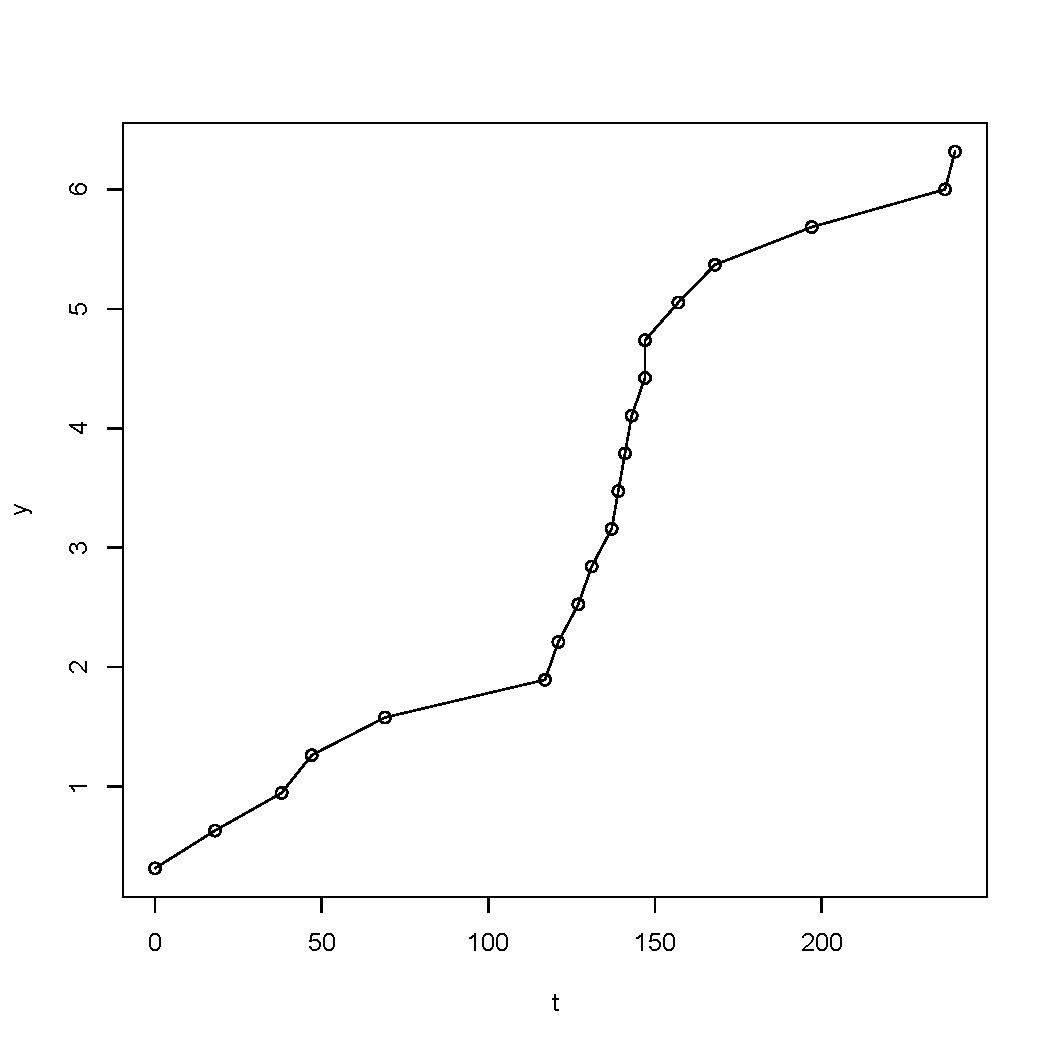
\includegraphics[scale = .5]{plot1.pdf}

%%%%%
%5
\item The following array gives us the values:

$\begin{array}{|c|c|}\hline
\tr{sacf} & \tr{acf}\\\hline
0.900721 & 0.901\\\hline
0.8208184 & 0.821\\\hline
0.7509325 & 0.751\\\hline
0.689028 & 0.689\\\hline
0.6363274 & 0.636\\\hline
0.5912949 & 0.591\\\hline
0.5500705 & 0.550\\\hline
0.5120536 & 0.512\\\hline
0.4786871 & 0.478\\\hline
0.4496129 & 0.449\\\hline
\end{array}$

I don't know about you, but I think that's pretty good.


\end{enumerate}

{\large Paper Summary}\\

The paper describes a nonparametric technique for estimating the cumulative intensity function $\Lambda(t)$ for a non-stationary Poisson poisson process on a finite time interval $(0,S]$.  The author starts by reviewing several proposed solutions for simulating NHPPs, such as thinning, assuming $\lambda(t)$ is of the form $(\alpha t)^\beta$, and estimating with a piecewise constant function.  Some flaws with these is that they are either computationally expensive or require arbitrary decisions from the modeler.  The author then suggests a procedure in which $\Lambda(t)$ is estimated with the following piecewise linear function determined by the order statistics of the superpositions of the $k$ realizations of the process:

$$\hat{\Lambda}(t) = \frac{in}{k(n+1)} + \frac{n(t - t_{(i)})}{(n+1)k(t_{(i+1)} - t_{(i)})}$$

The author then justifies the use of the proposed estimator, and proceeds to variate generation.  After that, the author describes examples.

\end{document}